\documentclass[hidelinks,a4paper,10pt, nofootinbib]{article}
\usepackage[width=15.5cm, left=3cm, top=2.5cm, right=2cm, left=2cm, height= 24.5cm]{geometry}
\usepackage[spanish]{babel}
\usepackage[utf8]{inputenc}
\usepackage[T1]{fontenc}
\usepackage{xspace}
\usepackage{xargs}
\usepackage{fancyhdr}
\usepackage{lastpage}
\usepackage{caratula}
\usepackage[bottom]{footmisc}
\usepackage{amssymb}
\usepackage{amsmath}
\usepackage{algorithm}
\usepackage[noend]{algpseudocode}
\usepackage{hyperref} % links en índice
\usepackage{tabularx} % tablas copadas

\usepackage{graphicx}
\usepackage{sidecap}
\usepackage{wrapfig}
\usepackage{caption}
\usepackage{tikz}

% facilitates the creation of memory maps. Start address at the bottom, end address at the top.
% syntax: \memsection{end address}{start address}{height in lines}{text in box}
\newcommand{\memsection}[4]{
\bytefieldsetup{bitheight=#3\baselineskip}    % define the height of the memsection
\bitbox[]{10}{
\texttt{#1}     % print end address
\\ \vspace{#3\baselineskip} \vspace{-2\baselineskip} \vspace{-#3pt} % do some spacing
\texttt{#2} % print start address
}
\bitbox{16}{#4} % print box with caption
}

\newcommand{\xmmdw}[5][]{
\begin{center}
\begin{tikzpicture}[xscale=1.15,yscale=.9]
	\draw [very thick, rounded corners] (0,0) rectangle (16, 1);
	\foreach \i in {4,8,12} {
		\draw (\i, 0) -- (\i, 1);
	}
	\node at (2,.5) {#2};
	\node at (6,.5) {#3};
	\node at (10,.5) {#4};
	\node at (14,.5) {#5};
	\node[below] at (8, 0) {\texttt{#1}};
	\node[below left] at (16, 0) {\footnotesize 0};
	\node[below right] at (0, 0) {\footnotesize 16};
\end{tikzpicture}
\end{center}
}

\newcommand{\xmmw}[8]{
\begin{center}
\begin{tikzpicture}[xscale=1.15,yscale=.7]
\draw [very thick, rounded corners] (0,0) rectangle (16, 1);
	\foreach \i in {2,4,6,8,10,12,14} {
		\draw (\i, 0) -- (\i, 1);
	}
	\node at (1,.5) {#1};
	\node at (3,.5) {#2};
	\node at (5,.5) {#3};
	\node at (7,.5) {#4};
	\node at (9,.5) {#5};
	\node at (11,.5) {#6};
	\node at (13,.5) {#7};
	\node at (15,.5) {#8};
	\node[below left] at (16, 0) {\footnotesize 0};
	\node[below right] at (0, 0) {\footnotesize 16};

\end{tikzpicture}
\end{center}
}

\newcommand\xmmb[1][]{%
	\def\xmmreg{#1}%
	\xmmbcont
}


\newcommand\xmmbcont[8]{%
    \def\tempa{#1}%
    \def\tempb{#2}%
    \def\tempc{#3}%
    \def\tempd{#4}%
    \def\tempe{#5}%
    \def\tempf{#6}%
    \def\tempg{#7}%
    \def\temph{#8}%
    \xmmbcontcont
}

\newcommand{\xmmbcontcont}[8]{
\begin{center}
\begin{tikzpicture}[xscale=1.15,yscale=.7]
	\draw [very thick, rounded corners] (0,0) rectangle (16, 1);
	\foreach \i in {1,...,15} {
		\draw (\i, 0) -- (\i, 1);
	}
	
	\node at (.5,.5) {\tempa};
	\node at (1.5,.5) {\tempb};
	\node at (2.5,.5) {\tempc};
	\node at (3.5,.5) {\tempd};
	\node at (4.5,.5) {\tempe};
	\node at (5.5,.5) {\tempf};
	\node at (6.5,.5) {\tempg};
	\node at (7.5,.5) {\temph};
	\node at (8.5,.5) {#1};
	\node at (9.5,.5) {#2};
	\node at (10.5,.5) {#3};
	\node at (11.5,.5) {#4};
	\node at (12.5,.5) {#5};
	\node at (13.5,.5) {#6};
	\node at (14.5,.5) {#7};
	\node at (15.5,.5) {#8};

	\node[below] at (8, 0) {\texttt{\xmmreg}};
	\node[below left] at (16, 0) {\footnotesize 0};
	\node[below right] at (0, 0) {\footnotesize 16};
\end{tikzpicture}
\end{center}
}

%%fancyhdr
\pagestyle{fancy}
\thispagestyle{fancy}
\addtolength{\headheight}{1pt}
\lhead{Organización del Computador II: TP2}
\rhead{$2º$ cuatrimestre de 2016}
\cfoot{\thepage\ / \pageref{LastPage}}
\renewcommand{\footrulewidth}{0.4pt}

%%caratula
\materia{Organización del Computador II}
\titulo{Trabajo Práctico II}
\subtitulo{Modelo de procesamiento SIMD}
\grupo{Grupo: El Arquitecto}
\integrante{Gatti, Mathias Nicolás}{477/14}{mathigatti@gmail.com}
\integrante{Pondal, Iván}{078/14}{ivan.pondal@gmail.com}
\integrante{Pondal, Iván}{078/14}{ivan.pondal@gmail.com}

\begin{document}
\tableofcontents

\newpage
\section{Introducción}
\par{Este trabajo propone observar las diferencias en los tiempos de cómputo debidas al aprovechamiento del modelo de procesamiento SIMD con respecto a implementaciones en C.}
\par{Se implementaron diversos filtros de los cuales se expone una breve explicación a continuación y luego se detallan en sus respectivas secciones.}
\begin{itemize}
\item[•] \textbf{Smalltiles:} genera una imagen del mismo tamaño de la original que la contiene 4 veces, una en cada cuadrante.
\item[•] \textbf{Rotar canales:} intercambia los colores de modo que lo azul pasa a ser rojo, lo rojo, verde y lo verde, azul.
\item[•] \textbf{Pixelar:} como su nombre lo indica, pixela la imagen disminuyendo la definición.
\item[•] \textbf{Combinar:} consiste en combinar 2 imágenes en función de un parámetro.
\item[•] \textbf{Colorizar:} intensifica los colores predominantes en cada píxel.
\end{itemize}

\begin{center}
 \begin{tabular}{cccc}
   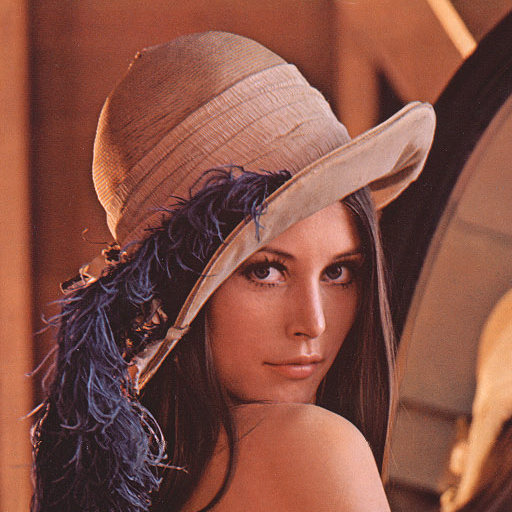
\includegraphics[width=0.2\textwidth]{imagenes/lena.png} &
   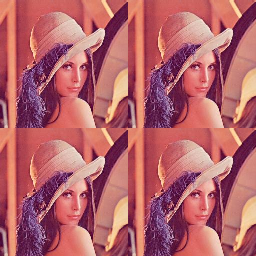
\includegraphics[width=0.2\textwidth]{imagenes/lena-smalltiles.png} &
   
\includegraphics[width=0.2\textwidth]{imagenes/lena-rotar-canales.png} \\
   Imagen original & Smalltiles & Rotar \\
   \\
   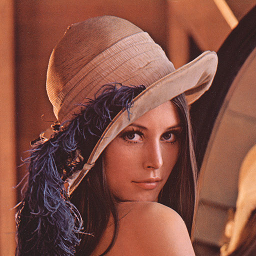
\includegraphics[width=0.2\textwidth]{imagenes/lena-pixelar.png} &
   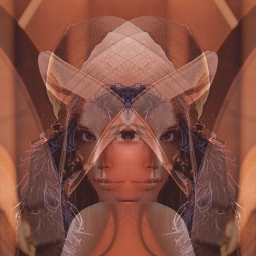
\includegraphics[width=0.2\textwidth]{imagenes/lena-combinar.png} &
   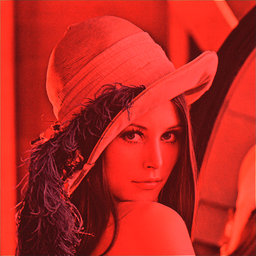
\includegraphics[width=0.2\textwidth]{imagenes/lena-colorizar.png} \\
   Pixelar & Combinar & Colorizar \\
 \end{tabular}
\end{center}

\par{Además de implementar los filtros en C y en Assembler se llevaron a cabo distintos experimentos para confirmar la hipótesis que motivó el trabajo, el hecho de que el procesamiento SIMD es más eficiente y permite resultados mucho más veloces que los obtenidos con las implementaciones de C.}

\newpage
\section{Rotar canales}
\par{El filtro consiste en una rotación de canales en cada píxel, como bien indica su nombre. Y la rotación se da de esta manera:}
\begin{center}
\textbf{R} $\longrightarrow$ \textbf{G}\\
\textbf{G} $\longrightarrow$ \textbf{B}\\
\textbf{B} $\longrightarrow$ \textbf{R}\\
\end{center}

\subsection{Código C}
\par{En el código de C recorremos la matriz iterando sus filas y columnas y modificando un píxel a la vez.
A continuación presentamos su pseudocódigo}

\begin{algorithm}[h!]
\caption{Rotar}
\begin{algorithmic}
  \Function{rotar}{src: *unsigned char, dst: *unsigned char, cols: int, filas: int, srcRowSize: int, dstRowSize: int}
	\State $unsigned~ char~ (*srcMatrix)[srcRowSize] = (unsigned~ char (*)[srcRowSize])~ src$
	\State $unsigned~ char~ (*dstMatrix)[dstRowSize] = (unsigned~ char (*)[dstRowSize])~ dst$
	\For{$f \gets 0~..~filas-1$}
		\For{$c \gets 0~..~cols-1$}
			\State $bgra_t* p_s \gets (bgra_t*)$ \& $srcMatrix[f][c * 4]$
			\State $bgra_t *p_d \gets (bgra_t*)$ \&$dstMatrix[f][c * 4]$
			
			\State $p_d \rightarrow$b $\gets$ $p_s \rightarrow g$
			\State $p_d \rightarrow$g $\gets$ $p_s \rightarrow r$
			\State $p_d \rightarrow$r $\gets$ $p_s \rightarrow b$
			\State $p_d \rightarrow$ a $\gets$ $p_s \rightarrow a$
		\EndFor
	\EndFor
\EndFunction
\end{algorithmic} 
\end{algorithm}
	
\subsection{Código ASM}
\par{El código de ASM recorre la matriz de la misma manera que la recorre el código de C, pero procesa 4 píxeles por iteración.}
\par{Las instrucciones propias de SIMD aceleran mucho el proceso y aportan mejoras considerables incluso al compararlo con un código de ASM sin utilizarlas.}

En cada ciclo se cargan 4 píxeles en xmm0 y se aplica \textbf{pshufb xmm0, xmm3}, donde este es:
\xmmb{$0f$}{$0c$}{$0e$}{$0d$}{$0b$}{$08$}{$0a$}{$09$}{$07$}{$04$}{$06$}{$05$}{$03$}{$00$}{$02$}{$01$}
Luego se guarda en memoria en la imagen destino, se incrementa el contador en 4 (procesamos 4 píxeles) y los respectivos punteros a las imagenes en 16 (4 píxeles ocupan 16 bytes).	
	
	
\subsection{Experimentación}

\subsubsection{Idea}	
\par{Para la experimentación con Rotar notamos la facilidad con la que se codea y procesa el filtro gracias a las instrucciones de SIMD, por ello quisimos ver si, además, generaban alguna optimización sobre un código sin estas herramientas.}
\par{Luego comparamos la eficiencia de ASM contra el código de C y distintas optimizaciones de este.}

\subsubsection{Hipótesis}
\par{La hipótesis que tuvimos sobre la primera idea era que efectivamente íbamos a notar un cambio ya que íbamos a estar procesando la mitad de píxeles por iteración. También suponíamos que iba a ser más complicado manipular los píxeles al no contar con instrucciones como \textbf{shuffle}, \textbf{unpacked}, \textbf{psrlx} y \textbf{psllx}.}
	
\subsubsection{Resultados}
\par{Efectivamente vimos una notoria diferencia entre el código en ASM con y sin SIMD, más aún, el código optimizado de C es más eficiente que éste último.}
\par{A continuación adjuntamos un gráfico en el que se puede apreciar dicha diferencia.}
	
\begin{figure}[H]
\centering
\captionsetup{justification=centering}
	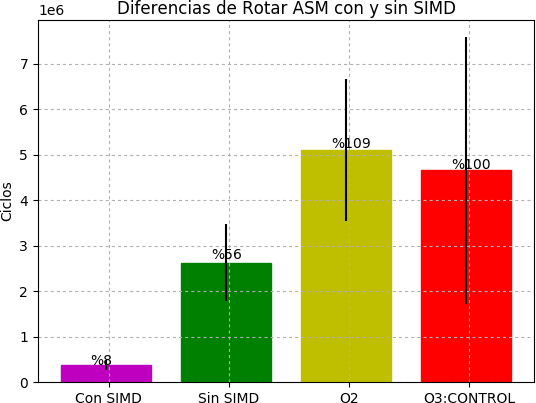
\includegraphics[width = 12 cm, height = 8 cm]{imagenes/RotarSinSIMD.png}
\caption[center]{Gráfico que compara las velocidad de las ejecuciones de las implementaciones con y sin el uso de instrucciones SSE, y también con optimizaciones de la implementación en C.}
\end{figure}

\par{El gráfico se armó en base a un conjunto de corridas de cada implementación del filtro, de donde se tomó la cantidad mínima de ciclos; con esto buscamos reducir la proporción de tiempo que consideramos que nuestro programa no estaba corriendo, si no que el scheduler estaba ejecutando otro programa.}\\
\par{A continuación mostramos un gráfico (armado de igual manera que el anterior) donde mostramos los tiempos de ejecución del filtro implementado en ASM y en C con distintas optimizaciones.}
	
\begin{figure}[H]
\centering
\captionsetup{justification=centering}
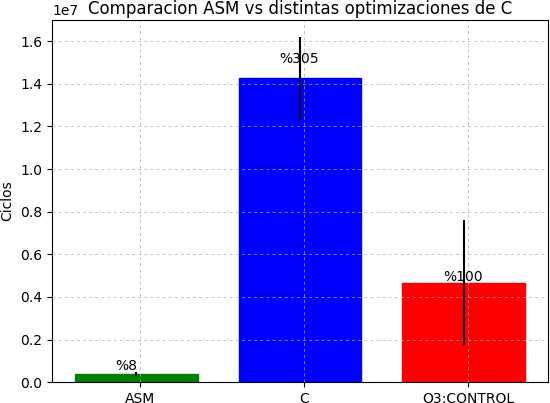
\includegraphics[width = 13 cm, height = 8 cm]{imagenes/ASMvsCRotar.png}
\caption[center]{Diferencias en cantidad de ciclos para la ejecución del filtro con la implementación en ASM y la de C con sus optimizaciones.}
\end{figure}

\newpage
\section{Smalltiles}
\par{Este filtro consiste en replicar 4 veces la imagen original achicada. De esta manera, si enumeramos los píxeles a partir del 0, siempre estaremos utilizando los píxeles de número par de la imagen original para generar las 4 más pequeñas.}
\subsection{Código C}
\par{En el código de C recorremos el equivalente a una de las 4 fotos pequeñas. En el píxel de la posición \emph{(i,j)} guardamos el contenido del de la posición \emph{(2*i,2*j)} en la imagen original. A la vez cargamos este contenido en las otras 3 imágenes.}
\par{A continuación mostramos el pseudocódigo de Smalltiles:}
\begin{algorithm}[h!]
\caption{Smalltiles}
\begin{algorithmic}
  \Function{smalltiles}{src: *unsigned char, dst: *unsigned char, cols: int, filas: int, srcRowSize: int, dstRowSize: int}
	\State $unsigned~ char~ (*srcMatrix)[srcRowSize] = (unsigned~ char (*)[srcRowSize])~ src$
	\State $unsigned~ char~ (*dstMatrix)[dstRowSize] = (unsigned~ char (*)[dstRowSize])~ dst$
	\State int ancho $\gets$ col/2
	\State int largo $\gets$ filas/2
	\For{$f \gets 0~..~largo-1$}
		\For{$c \gets 0~..~ancho-1$}
			\State $bgra_t* p_s \gets (bgra_t*)$ \& $srcMatrix[f][c * 4]$
			\For{$i \gets 0~..~1$}		
				
				\State $bgra_t *p_d \gets (bgra_t*)$ \&$dstMatrix[f][(c + ancho*i) * 4]$
				
				\State ($p_d \rightarrow$b) $\gets$ ($p_s \rightarrow b$)
				\State ($p_d \rightarrow$g) $\gets$ ($p_s \rightarrow g$)
				\State ($p_d \rightarrow$r) $\gets$ ($p_s \rightarrow r$)
				\State ($p_d \rightarrow$ a) $\gets$ ($p_s \rightarrow a$)
			\EndFor
			\For{$i \gets 0~..~1$}		
				
				\State $bgra_t *p_d \gets (bgra_t*)$ \&$dstMatrix[f + largo][c * 4]$
				
				\State ($p_d \rightarrow$b) $\gets$ ($p_s \rightarrow b$)
				\State ($p_d \rightarrow$g) $\gets$ ($p_s \rightarrow g$)
				\State ($p_d \rightarrow$r) $\gets$ ($p_s \rightarrow r$)
				\State ($p_d \rightarrow$ a) $\gets$ ($p_s \rightarrow a$)
			\EndFor
		\EndFor
	\EndFor
\EndFunction

\end{algorithmic} 
\end{algorithm}
	
\subsection{Código ASM}
\par{En la implementación de ASM recorremos las filas de la imagen; tenemos dos ciclos, el interno recorre una fila iterando sobre sus columnas, y el externo itera sobre todas las filas de la imagen.}
\par{En el ciclo interno cargamos 8 píxeles, nos encargamos de ubicarlos en un registro xmmi a nuestra conveniencia utilizando \textbf{pshufd}, \textbf{psrldq}, \textbf{pslldq} y \textbf{paddb}.}
\par{En un principio cargamos los primeros 4 píxeles en \textbf{xmm1} y luego \textbf{pshud xmm1, xmm1,0xd8}.}
	\textbf{xmm1:}
	\xmmdw{$pixel4$}{$pixel2$}{$pixel3$}{$pixel1$}
	Luego cargamos los siguientes 4 píxeles en xmm10 y también \textbf{pshud xmm10,xmm10, 0x2d}.\\
	\textbf{xmm10:}
	\xmmdw{$pixel5$}{$pixel7$}{$pixel8$}{$pixel6$}
	Luego shifteamos convenientemente y sumamos los xmmi.\\
	\textbf{xmm10:}
	\xmmdw{$pixel8$}{$pixel6$}{$pixel4$}{$pixel2$}
	Ya tenemos en \textbf{xmm10} la información tal cual queremos guardarla, ahora simplemente la guardamos en memoria manipulando algunos ínidices para cargarla en los 4 cuadrantes de la imagen destino.
	
\subsection{Experimentación}

\subsubsection{Idea}
\par{Nuestra implementación de ASM consiste en un ciclo que itera sobre las filas, por ende tuvimos la idea de experimentar sobre eso. Es decir, la cantidad de filas es un factor clave que influye bastante en la cantidad de ciclos de ejecución del filtro. Entonces nuestro experimento se basó en analizar los distintos tiempos de ejecución de imágenes con igual cantidad de píxeles totales, pero con distinto ancho y largo.}

\subsubsection{Hipótesis}
\par{Al comparar dos imágenes donde el ancho de una es la altura de la otra y viceversa, la aplicación del filtro a la imagen con menor altura tomaría menos ciclos. Cuanto más cercanos sean los valores de altura y ancho, menos varía la cantidad de ciclos.}
	
\subsubsection{Resultados}
\par{Efectivamente eso es lo que podemos observar en el siguiente gráfico. La cantidad de ciclos varía más en las imágenes de 200x1600 y 1600x200, donde podemos observar una diferencia de más de 4 millones de ciclos. En cambio en el par de imágenes de 640x500 y 500x640 la diferencia es de tan solo \textcolor{red}{1 millón y medio} (exactamente \textcolor{red}{155981} ciclos). Estos experimentos se realizaron con la misma imagen rotada y sin rotar, aunque en el caso de este filtro, las cualidades de los píxeles no modifican los resultados.}

\begin{figure}[H]
\centering
\captionsetup{justification=centering}
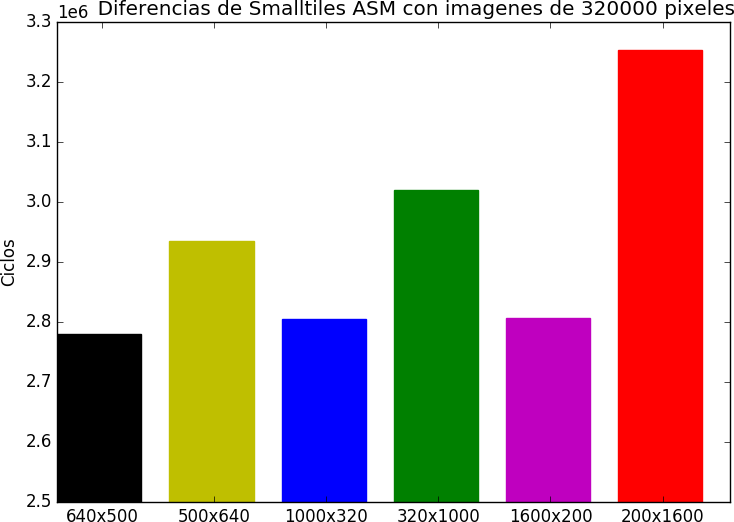
\includegraphics[width = 15 cm, height = 10 cm]{imagenes/distintostamanos.png}
\caption[center]{Gráfico de barras que da cuenta de los ciclos que implica cada corrida del filtro para imágenes de distintos tamaños con una determinada cantidad fija de píxeles.}
\end{figure}
	
\par{A continuación adjuntamos el gráfico que compara la cantidad de ciclos que tarda en ejecutarse el filtro implementado en ASM y el implementado en C.}

\begin{figure}[h!]
\centering
\captionsetup{justification=centering}
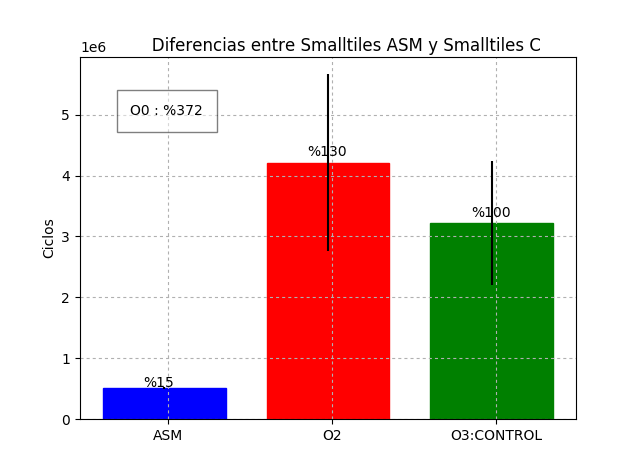
\includegraphics[width = 15 cm, height = 12 cm]{imagenes/ASMvsCSmalltiles.png}
\caption[center]{Comparación de las implementaciones y compilaciones con distintos niveles de optimización en cuanto a la rapidez para el procesamiento de una imagen.}
\end{figure}
	

\newpage
\section{Pixelar}
Este filtro consiste en tomar bloques de 2x2 píxeles y asignarles a estos el promedio del bloque. De esta manera se disminuye la cálidad de la imágen.
\subsection{Código C}
	El código de C consiste en recorrer la imagen de a dos filas y dos columnas por iteración. En cada iteración se calcula el promedio de los canales de los píxeles.
	A continuación adjuntamos el pseudocódigo.

\begin{algorithm}[h!]
\caption{Promedio}
\begin{algorithmic}
  \Function{promedio}{$a :~unsigned~ char, ~b:~ unsigned ~char, ~c: ~unsigned~ char, ~d: ~unsigned~ char$}  $\to \texttt{float}$
	\State $float~ af \gets a$
	\State $float~ bf \gets b$
	\State $float~ cf \gets c$
	\State $float~ df \gets d$
	\State \Return $(af/4+bf/4+cf/4+df/4)$
	
\EndFunction
\end{algorithmic} 
\end{algorithm}	
	
	\begin{algorithm}[h!]
\caption{Pixelar}
\begin{algorithmic}
  \Function{pixelar}{src: *unsigned char, dst: *unsigned char, cols: int, filas: int, srcRowSize: int, dstRowSize: int}
	\State $unsigned~ char~ (*srcMatrix)[srcRowSize] = (unsigned~ char (*)[srcRowSize])~ src$
	\State $unsigned~ char~ (*dstMatrix)[dstRowSize] = (unsigned~ char (*)[dstRowSize])~ dst$
	
	\For{$f \gets 0~..~filas-1; f+=2$}
		\For{$c \gets 0~..~cols-1; c+=2$}
			\State $bgra_t* p_s1 \gets (bgra_t*)$ \& $srcMatrix[f][c * 4]$
			\State $bgra_t *p_d1 \gets (bgra_t*)$ \&$dstMatrix[f][c * 4]$
			
			\State $bgra_t* p_s2 \gets (bgra_t*)$ \& $srcMatrix[f+1][c * 4]$
			\State $bgra_t *p_d2 \gets (bgra_t*)$ \&$dstMatrix[f+1][c * 4]$
			
			\State $bgra_t* p_s3 \gets (bgra_t*)$ \& $srcMatrix[f+1][(c+1) * 4]$
			\State $bgra_t *p_d3 \gets (bgra_t*)$ \&$dstMatrix[f+1][(c+1) * 4]$
			
			\State $bgra_t* p_s4 \gets (bgra_t*)$ \& $srcMatrix[f][(c+1) * 4]$
			\State $bgra_t *p_d4 \gets (bgra_t*)$ \&$dstMatrix[f][(c+1) * 4]$
			
			\State k $\gets$ 0.5
			
			\State b $\gets$ \Call{promedio}{$p_s \rightarrow b, p_s2 \rightarrow b, p_s3 \rightarrow b, p_s4 \rightarrow b$}
			\State g $\gets$ \Call{promedio}{$p_s \rightarrow g, p_s2 \rightarrow g,p_s3 \rightarrow g, p_s4 \rightarrow g$}
			\State r $\gets$ \Call{promedio}{$p_s \rightarrow r, p_s2 \rightarrow r, p_s3 \rightarrow r, p_s4 \rightarrow r$}
			\State a $\gets$ \Call{promedio}{$p_s \rightarrow a, p_s2 \rightarrow a, p_s3 \rightarrow a, p_s4 \rightarrow a$}
				
			\For{$i \gets 1~..~4$}
				\State ($p_di \rightarrow$b) $\gets$ b
				\State ($p_di \rightarrow$g) $\gets$ g
				\State ($p_di \rightarrow$r) $\gets$ r
				\State ($p_di \rightarrow$ a) $\gets$ a
			\EndFor
		\EndFor
	\EndFor
\EndFunction

\end{algorithmic} 
\end{algorithm}
\subsection{Código ASM}
El codigo en ASM consiste en una union de cilos, uno exterior para iterar sobre las filas y otro interior para iterar sobre los elemntos de la misma (columnas). Lo que hace este codigo es en cada iteracion, lee de memoria dos veces, empezando en la misma columna pero de dos filas diferentes. De esta forma levanta como una matriz de 8 elementos (4x2). Lo que se puede obtener de esta informacion va a servir para sobre escribir 8 pixeles. \\ El ciclo luego procede en exteneder los signos de cada byte, luego guardar la sumatoria de los elementos {1,2,6,7} (mirandolo como una matriz de 4x2), y la sumatoria de {4,5,8,9} en dos registros aparte, calcular el promedio de esto, osea dividirlos por cuatro. Y luego a esta informacion la volvemos a agrupar juntas en un mismo registro que se veria de esta manera :

\par{\textbf{XMM:}}
\xmmb{$Pp1_a$}{$Pp1_r$}{$Pp1_g$}{$Pp1_b$}{$Pp1_a$}{$Pp1_r$}{$Pp1_g$}{$Pp1_b$}{$Pp2_a$}{$Pp2_r$}{$Pp2_g$}{$Pp2_b$}{$Pp2_a$}{$Pp2_r$}{$Pp2_e$}{$Pp2_b$}
\par {Pp1 : promedio pixeles {1,2,6,7}. Pp2 : promedio pixeles {4,5,8,9}}
	
	
.\\ Y finalmente a este registro lo escribimos en la imagen destino, en los lugar de los cual levantamos en la imagen src. \\ Por ultimo movemos los current en columnas 4 pixeles que es la cantidad sobre esa fila q procesamos en cada iteracion. Y si terminamos de procesar la fila, nos movemos dos filas, ya que vamos procesando dos juntas a la vez.
	
\subsection{Experimentación 1}
\subsubsection{Idea}	
	Comparamos la eficacia del código en ASM contra C y C optimizado.
	
\subsubsection{Resultados}
	\begin{figure}[h!]
	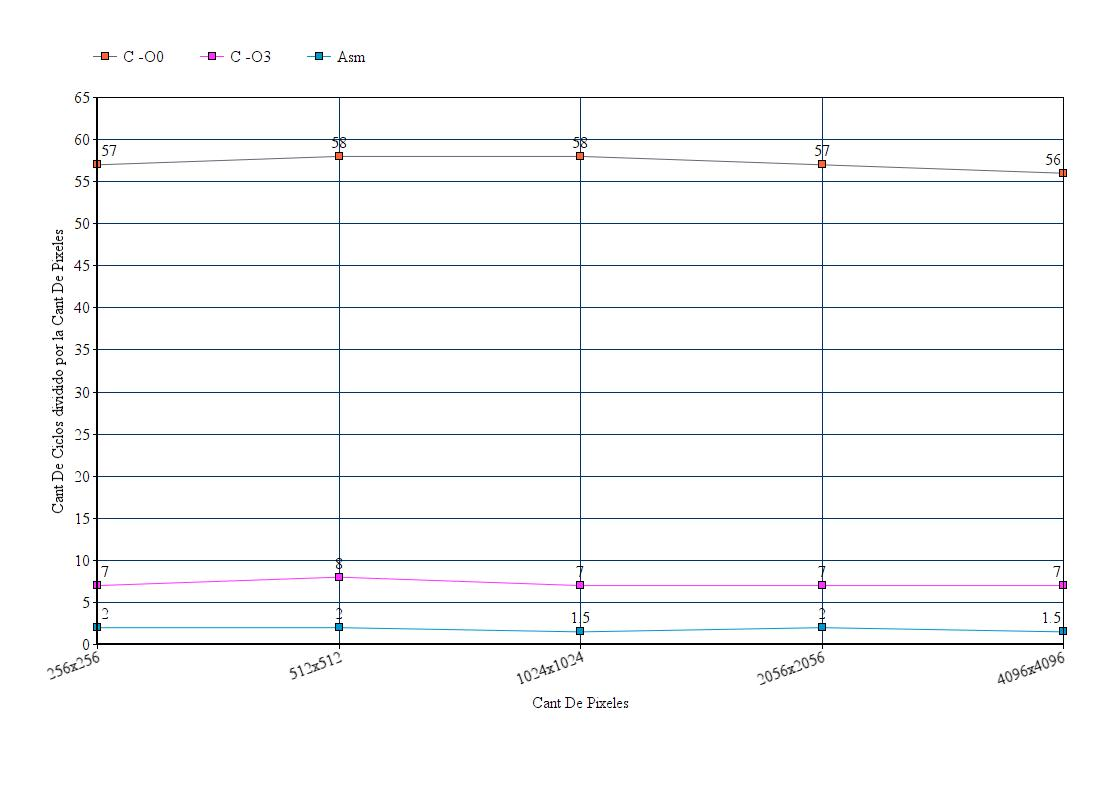
\includegraphics[width = 15 cm, height = 10 cm]{imagenes/pixeAsmC.png}
	\caption[center]{Comparacion (ciclos Totales) / (cant De pixeles) - diferentes Implementaciones de C y Asm}
\end{figure}

\subsection{Experimentacion 2}
\subsubsection{Idea}
Comparamos la eficacia entre utilizar instrucciones como shift, para dividir los pixeles, contra las instrucciones para dividir floats, que implican ademas tener que hacer un traspaso de formato.

\subsubsection{Hipotesis}
Nuestra idea es que va a ser mucho mas optimo el codigo donde utilizamos las intrucciones de shift para dividir los nunmeros, porque son operaiones basicas que se encarga el registro de hacerlas, en cambio el pasar a float, dividir luego y volver  a pasar a float, son todas operaciones sin implementacion primitiva, osea por esto nos referimos a que estan compuestas de varias otras instrucciones y hace que la ejecucion de cada una demore varios ciclos mas que un simple shift.

\subsubsection{Resultados}
	\begin{figure}[!h]
	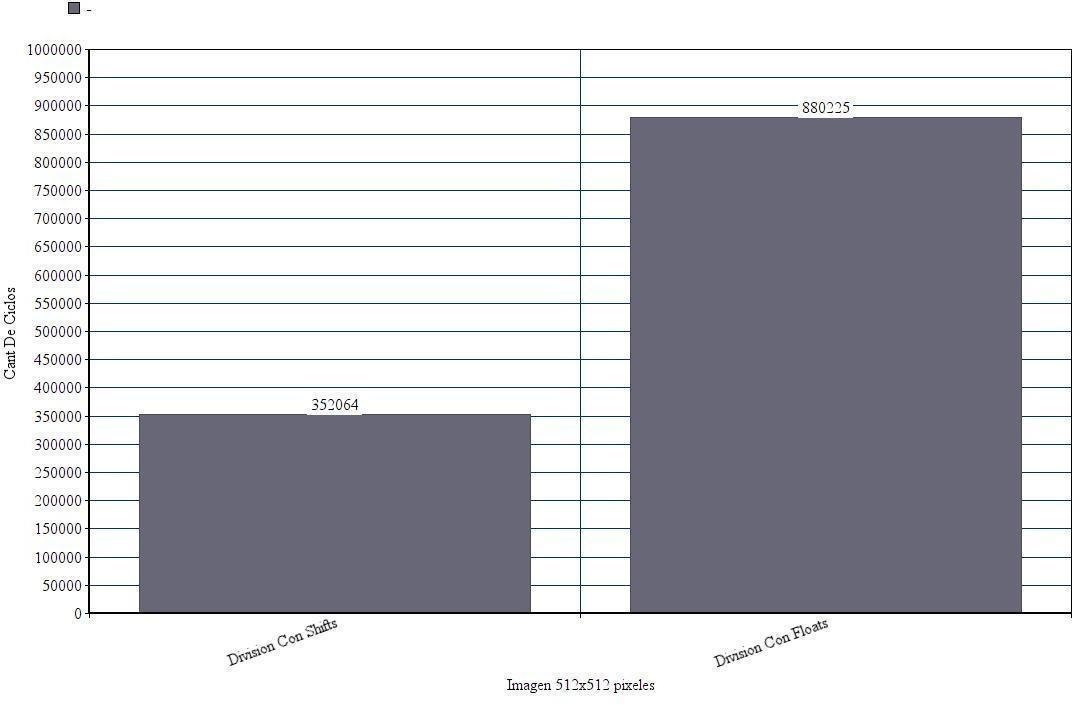
\includegraphics[width = 15 cm, height = 10 cm]{imagenes/Div_pixelar.jpg}
	\end{figure}
	
\subsubsection{Conclucion}
	Definitivamente el codigo en el cula dividimos con shifts fue mucho mas optimo, denuevo por lo que explicamos en la hipotesis.

\newpage
\section{Combinar}
\par{Este filtro consiste en realizar una combinación de dos imágenes que dependa de un número real $\alpha$ entre 0 y 255.}
\par{Cabe destacar que este filtro permite reutilizar cálculos debido a dos factores. Uno de ellos es la forma que tiene cada píxel generado en la imagen resultante, que consiste en que si se tienen una imagen $A$ y una imagen $B$ de tamaño $m \times n$ entonces el píxel de la imagen generada ${I_{AB}}^{i, j}$ se calcula de la siguiente forma:}
\[ {I_{AB}}^{i,j} = \dfrac{\alpha * ( {I_{A}}^{i,j} - {I_{B}}^{i,j} )}{255.0} + {I_{B}}^{i,j} \]
\par{El otro factor es que nuestro filtro está optimizado para casos en los que la imagen $B$ es el reflejo vertical de la imagen $A$. Es decir que se da que ${I_{A}}^{i,j} = {I_{B}}^{i,n - j + 1}$ como se puede apreciar en la siguiente figura.}

\begin{figure}[h!]
\centering
\begin{minipage}{.5\textwidth}
\centering
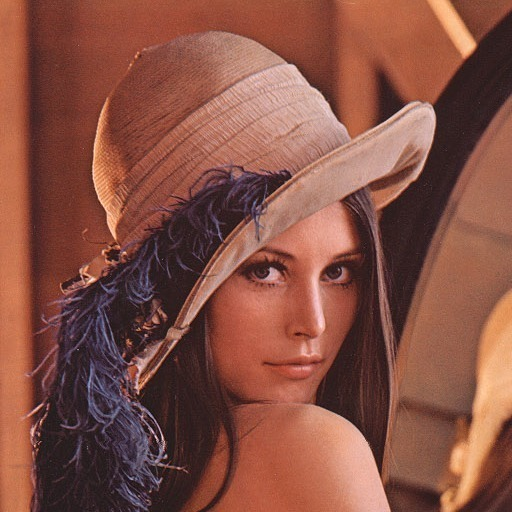
\includegraphics[width=5cm, height=5cm]{imagenes/CombinarOriginal.jpg}
\label{}
\end{minipage}\hfill
\begin{minipage}{.5\textwidth}
\centering
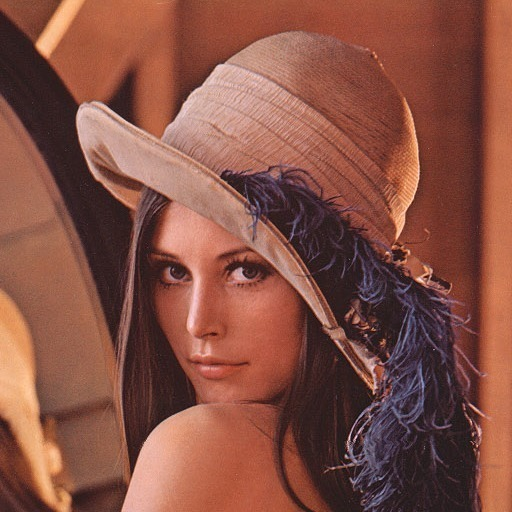
\includegraphics[width=5cm, height=5cm]{imagenes/CombinarReflejo.jpg}
\label{}
\end{minipage}
\caption[center]{Se muestra la imagen $A$ del lado izquierdo con la imagen $B$, el reflejo vertical de A, en la parte derecha.}
\end{figure}

\par{Entonces se tiene que}
\begin{align}
{I_{AB}}^{i,j} &= \dfrac{\alpha * ( {I_{A}}^{i,j} - {I_{B}}^{i,j} )}{255.0} + {I_{B}}^{i,j} \textup{     por la fórmula del filtro} \nonumber \\
&= \dfrac{\alpha * ( {I_{A}}^{i,j} - {I_{A}}^{i,n - j + 1} )}{255.0} + {I_{A}}^{i,n - j + 1} \textup{    dado que} {I_{A}}^{i,j} = {I_{B}}^{i,n - j + 1}
\end{align}

y análogamente

\begin{align}
{I_{AB}}^{i,n - j + 1} &= \dfrac{\alpha * ( {I_{A}}^{i,n - j + 1} - {I_{B}}^{i,n - j +1} )}{255.0} + {I_{B}}^{i,n - j + 1}  \nonumber \\
&= \dfrac{\alpha * ( {I_{A}}^{i,n - j + 1} - {I_{A}}^{i,j} )}{255.0} + {I_{A}}^{i,j}
\end{align}

\par{Así, se obtiene}

\begin{align}
{I_{AB}}^{i,n - j + 1} &= -1 * \dfrac{\alpha * [-1 * ( {I_{A}}^{i,n - j + 1} - {I_{A}}^{i,j} )]}{255.0} - {I_{A}}^{i,n - j + 1} + {I_{A}}^{i,n - j + 1} + {I_{A}}^{i,j} \nonumber \\
&= -1 * \Big[ \dfrac{\alpha * ( {I_{A}}^{i,j} - {I_{A}}^{i,n - j + 1} )}{255.0} + {I_{A}}^{i,n - j + 1} \Big] + {I_{A}}^{i,n - j + 1} + {I_{A}}^{i,j} \nonumber \\
&= -1 * ( {I_{AB}}^{i,j} - {I_{A}}^{i,n - j + 1} ) + {I_{A}}^{i,j} \textup{usando la igualdad de (2)}
\end{align}

\par{Estos cálculos muestran que luego de hacer el procesamiento para generar un píxel de la parte izquierda de la imagen resultante se puede obtener el píxel que corresponde a la mitad derecha con pocos cálculos más. Más aún, si se denomina}
\[ P = \dfrac{\alpha * ( {I_{A}}^{i,j} - {I_{A}}^{i,n - j + 1} )}{255.0} \]
se consigue
\[ {I_{AB}}^{i,j} = P + {I_{A}}^{i,n - j + 1} \]
y
\[ {I_{AB}}^{i,n - j + 1} = -P + {I_{A}}^{i,j} \]
dando lugar a menos cálculos necesarios.

\subsection{Código C}
\par{A continuación se presenta el pseudocódigo detallado del filtro.}
\par{Clamp es una función que controla la saturación.}
\begin{algorithm}[h!]
\caption{Clamp}
\begin{algorithmic}
  \Function{clamp}{$pixel: ~float$}  $\to \texttt{float}$
	\If{$pixel < 0.0$}
		\State \Return $0.0$
	\Else
		\If{$pixel > 255.0$}
			\State \Return $255.0$
		\Else
			\State \Return $pixel$
		\EndIf
	\EndIf
\EndFunction
\end{algorithmic} 
\end{algorithm}

\par{Combine realiza los cálculos correspondientes determinados por el filtro.}
\begin{algorithm}[h!]
\caption{Combine}
\begin{algorithmic}
  \Function{combine}{$a: ~unsigned~ char, ~b: ~unsigned~ char, ~\alpha: ~float$}  $\to \texttt{float}$
	\State float $af \gets a$
	\State float $bf \gets b$
	\State \Return $\dfrac{\alpha * (af - bf)}{255.0} + bf$
\EndFunction
\end{algorithmic} 
\end{algorithm}

\par{Combinar llama a las dos funciones ya explicadas y obtiene 2 píxeles con los que operar para luego dejar el resultado en la imagen destino.}
\begin{algorithm}[h!]
\caption{Combinar}
\begin{algorithmic}
  \Function{combinar}{src: *unsigned char, dst: *unsigned char, cols: int, filas: int, srcRowSize: int, dstRowSize: int, $\alpha$: float}
	\State $unsigned~ char~ (*srcMatrix)[srcRowSize] = (unsigned~ char (*)[srcRowSize])~ src$
	\State $unsigned~ char~ (*dstMatrix)[dstRowSize] = (unsigned~ char (*)[dstRowSize])~ dst$
	\For{$f \gets 0~..~filas-1$}
		\For{$c \gets 0~..~cols-1$}
			\State $bgra_t* p_{sa} \gets (bgra_t*)$ \& $srcMatrix[f][c * 4]$
			\State $bgra_t* p_{sb} \gets (bgra_t*)$ \&$srcMatrix[f][(cols - c -1) * 4]$
			\State $bgra_t *p_d \gets (bgra_t*)$ \&$dstMatrix[f][c * 4]$
			\State $p_d$->$b \gets$ \Call{clamp}{\Call{combine}{$p_{sa}$->$b$, $p_{sb}$->$b, \alpha$}}
			\State $p_d$->$g \gets$ \Call{clamp}{\Call{combine}{$p_{sa}$->$g, p_{sb}$->$g, \alpha$}}
			\State $p_d$->$r \gets$ \Call{clamp}{\Call{combine}{$p_{sa}$->$r, p_{sb}$->$r, \alpha$}}
			\State $p_d$->$a \gets$ \Call{clamp}{\Call{combine}{$p_{sa}$->$a, p_{sb}$->$a, \alpha$}}
		\EndFor
	\EndFor
\EndFunction
\end{algorithmic} 
\end{algorithm}
	
\subsection{Código ASM}
\par{Dado que cada píxel tiene 4 bytes y los registros XMM tienen 16 bytes, se levantan 4 píxeles contiguos desde la posición $i,j$ y otros 4 píxeles desde la $i, n-j+1$ en otro registro.}
\par{Se mostrará cómo se genera el píxel $I_{i,j}$ de la imagen resultante.}
%\xmmb{$P_{j+3}A$}{$P_{j+3}R$}{$P_{j+3}G$}{$P_{j+3}B$}{$P_{j+2}A$}{$P_{j+2}R$}{$P_{j+2}G$}{$P_{j+2}B$}{$P_{j+1}A$}{$P_{j+1}R$}{$P_{j+1}G$}{$P_{j+1}B$}{$P_jA$}{$P_jR$}{$P_jG$}{$P_jB$}
\par{Se levantan 4 píxeles de la mitad izquierda en el registro XMM1:}
\par{\textbf{XMM1:}}
\xmmb{$A_{j+3}$}{$R_{j+3}$}{$G_{j+3}$}{$B_{j+3}$}{$A_{j+2}$}{$R_{j+2}$}{$G_{j+2}$}{$B_{j+2}$}{$A_{j+1}$}{$R_{j+1}$}{$G_{j+1}$}{$B_{j+1}$}{$A_j$}{$R_j$}{$G_j$}{$B_j$}
\par{y 4 en espejo de la mitad derecha en XMM3:}\\
\par{\textbf{XMM3:}}
\xmmb{$A_{n-j+4}$}{$R_{n-j+4}$}{$G_{n-j+4}$}{$B_{n-j+4}$}{$A_{n-j+3}$}{$R_{n-j+3}$}{$G_{n-j+3}$}{$B_{n-j+3}$}{$A_{n-j+2}$}{$R_{n-j+2}$}{$G_{n-j+2}$}{$B_{n-j+2}$}{$A_{n-j+1}$}{$R_{n-j+1}$}{$G_{n-j+1}$}{$B_{n-j+1}$}

Teniendo
\par{\textbf{XMM9:}}
\xmmb{$0$}{$0$}{$0$}{$0$}{$0$}{$0$}{$0$}{$0$}{$0$}{$0$}{$0$}{$0$}{$0$}{$0$}{$0$}{$0$}
se ejecuta la instrucción \textbf{punpcklbw xmm1, xmm9} que da como resultado
\par{\textbf{XMM1:}}
\xmmb{$0$}{$A_{j+1}$}{$0$}{$R_{j+1}$}{$0$}{$G_{j+1}$}{$0$}{$B_{j+1}$}{$0$}{$A_j$}{$0$}{$R_j$}{$0$}{$G_j$}{$0$}{$B_j$}
\par{y luego \textbf{punpcklwd xmm1, xmm9} para seguir desempaquetando. De esta forma quedan 4 bytes para cada componente del píxel y se podrán convertir a floats para mayor precisión en los cálculos que implican el $\alpha$.}
\par{\textbf{XMM1:}}
\xmmb{$0$}{$0$}{$0$}{$A_j$}{$0$}{$0$}{$0$}{$R_j$}{$0$}{$0$}{$0$}{$G_j$}{$0$}{$0$}{$0$}{$B_j$}
\par{Se copió el contenido de XMM1 a XMM10 y con el registro que contenía al píxel $n-j+4$, obtenido de forma análoga a como se obtuvo el píxel $j$}
\par{\textbf{XMM8:}}
\xmmb{$0$}{$0$}{$0$}{$A_{n-j+4}$}{$0$}{$0$}{$0$}{$R_{n-j+4}$}{$0$}{$0$}{$0$}{$G_{n-j+4}$}{$0$}{$0$}{$0$}{$B_{n-j+4}$}
\par{se realizaron las restas entre componentes (\textbf{psubd xmm10, xmm8}) antes de convertir a float el registro XMM10 (\textbf{cvtdq2ps xmm10, xmm10}) dado que realizar la resta con float es una operación mucho más costosa que con enteros y además no había chances de perder precisión con la resta.}
\par{\textbf{XMM10:}}
\xmmdw{$A_j - A_{n-j+4}$}{$R_j - R_{n-j+4}$}{$G_j - G_{n-j+4}$}{$B_j - B_{n-j+4}$}
\par{Se multiplicó por $\alpha$ al registro XMM10 (\textbf{mulps xmm10, xmm0}) y luego se dividió por $255.0$ (\textbf{divps xmm10, xmm14}) obteniéndose}
\par{\textbf{XMM10:}}
\xmmdw{$\dfrac{\alpha * (A_j - A_{n-j+4})}{255.0}$}{$\dfrac{\alpha * (R_j - R_{n-j+4})}{255.0}$}{$\dfrac{\alpha * (G_j - G_{n-j+4})}{255.0}$}{$\dfrac{\alpha * (B_j - B_{n-j+4})}{255.0}$}
\par{Para esto previamente, fuera del ciclo, se había movido el $\alpha$ que había llegado en los últimos 4 bytes de XMM0 a las otras 3 double words del registro con la instrucción \textbf{pshufd xmm0, xmm0, 00000000b} y se había puesto en XMM14 un 255.0 en cada double word declarando \textbf{mascara255: dd 255.0, 255.0, 255.0, 255.0} en \textbf{section .rodata} y luego haciendo \textbf{movdqu xmm14, [mascara255]}. De esta forma, al realizar estas operaciones fuera del ciclo, se minimizan los accesos a memoria y se evita repetir operaciones innecesarias.}
\par{Convirtiendo XMM8 a float con \textbf{cvtdq2ps xmm8, xmm8} y sumándolo a XMM10 con \textbf{addps xmm10, xmm8} se obtuvo}
\par{\textbf{XMM10:}}
\xmmdw{$\dfrac{\alpha * (A_j - A_{n-j+4})}{255.0} + A_{n-j+4}$}{$\dfrac{\alpha * (R_j - R_{n-j+4})}{255.0} + R_{n-j+4}$}{$\dfrac{\alpha * (G_j - G_{n-j+4})}{255.0} + G_{n-j+4}$}{$\dfrac{\alpha * (B_j - B_{n-j+4})}{255.0} + B_{n-j+4}$}
\par{Antes de finalizar el procesamiento, se realizó \textbf{movups xmm15, xmm10} y \textbf{subps xmm15, xmm8} para conservar en XMM15 lo que en el desarrollo de cuentas apareció como P al explicar cómo se podían reutilizar cálculos.}
\par{Por último en el procesamiento de la parte izquierda se convirtió a entero XMM10 con \textbf{cvtps2dq xmm10, xmm10} y se empaquetó con los resultados de los demás píxeles usando instrucciones como \textbf{packusdw xmm11, xmm10} y \textbf{packusdw xmm13, xmm12} para pasar de double word a word,}
\par{\textbf{XMM11:}}
\xmmw{${F_A}_j$}{${F_R}_j$}{${F_G}_j$}{${F_B}_j$}{${F_A}_{j+1}$}{${F_R}_{j+1}$}{${F_G}_{j+1}$}{${F_B}_{j+1}$}
\par{luego \textbf{packuswb xmm13, xmm11} para pasar de word a byte,}
\par{\textbf{XMM11:}}
\xmmb{${F_A}_j$}{${F_R}_j$}{${F_G}_j$}{${F_B}_j$}{${F_A}_{j+1}$}{${F_R}_{j+1}$}{${F_G}_{j+1}$}{${F_B}_{j+1}$}{${F_A}_{j+2}$}{${F_R}_{j+2}$}{${F_G}_{j+2}$}{${F_B}_{j+2}$}{${F_A}_{j+3}$}{${F_R}_{j+3}$}{${F_G}_{j+3}$}{${F_B}_{j+3}$}
\par{y finalmente \textbf{pshufd xmm11, xmm13, 0x1b} quedando todo listo para mover el contenido del registro a donde correspondiera.}
\par{\textbf{XMM11:}}
\xmmb{${F_A}_{j+3}$}{${F_R}_{j+3}$}{${F_G}_{j+3}$}{${F_B}_{j+3}$}{${F_A}_{j+2}$}{${F_R}_{j+2}$}{${F_G}_{j+2}$}{${F_B}_{j+2}$}{${F_A}_{j+1}$}{${F_R}_{j+1}$}{${F_G}_{j+1}$}{${F_B}_{j+1}$}{${F_A}_j$}{${F_R}_j$}{${F_G}_j$}{${F_B}_j$}
\par{Para finalizar la parte derecha se multiplicaron todos los valores de las double words de XMM15 por -1 (\textbf{mulps xmm15, [menos1]} estando menos1 definido en \textbf{rodata} como \textbf{menos1: dd -1.0, -1.0, -1.0, -1.0}) y se prosiguió con las conversiones y sumas como anteriormente.}

	
\subsection{Experimentación}

\subsubsection{Hipótesis}
\par{Nuestra hipótesis era que la implementación en ASM iba a ser mucho más veloz que la de C con el menor nivel de optimización al compilar e incluso que las de C con mayores niveles de optimización.}
\par{Además creíamos que las ejecuciones con la implementación de C iban a presentar un porcentaje de ciclos de clock debidos accesos a memoria mucho mayor que la implementación de ASM.}

\subsubsection{Idea}
\par{Como forma de verificar esto pensamos medir la cantidad de ciclos de clock insumidos en cada caso para la ejecución del filtro. Se realizaron 1000 mediciones y se realizó un gráfico de barras con los promedios obtenidos de dividir cada total de ciclos por la cantidad de iteraciones.}
\par{Por otro lado, se midieron los ciclos de clock relacionados a accesos a memoria con la implementación de ASM y con la de C y se realizaron gráficos de torta para mostrar los porcentajes con respecto al total de ciclos insumidos.}

\subsubsection{Resultados}
\par{En cuanto a las cantidades totales de ciclos de clock se obtuvo el siguiente gráfico.}

\begin{figure}[h!]
\centering
	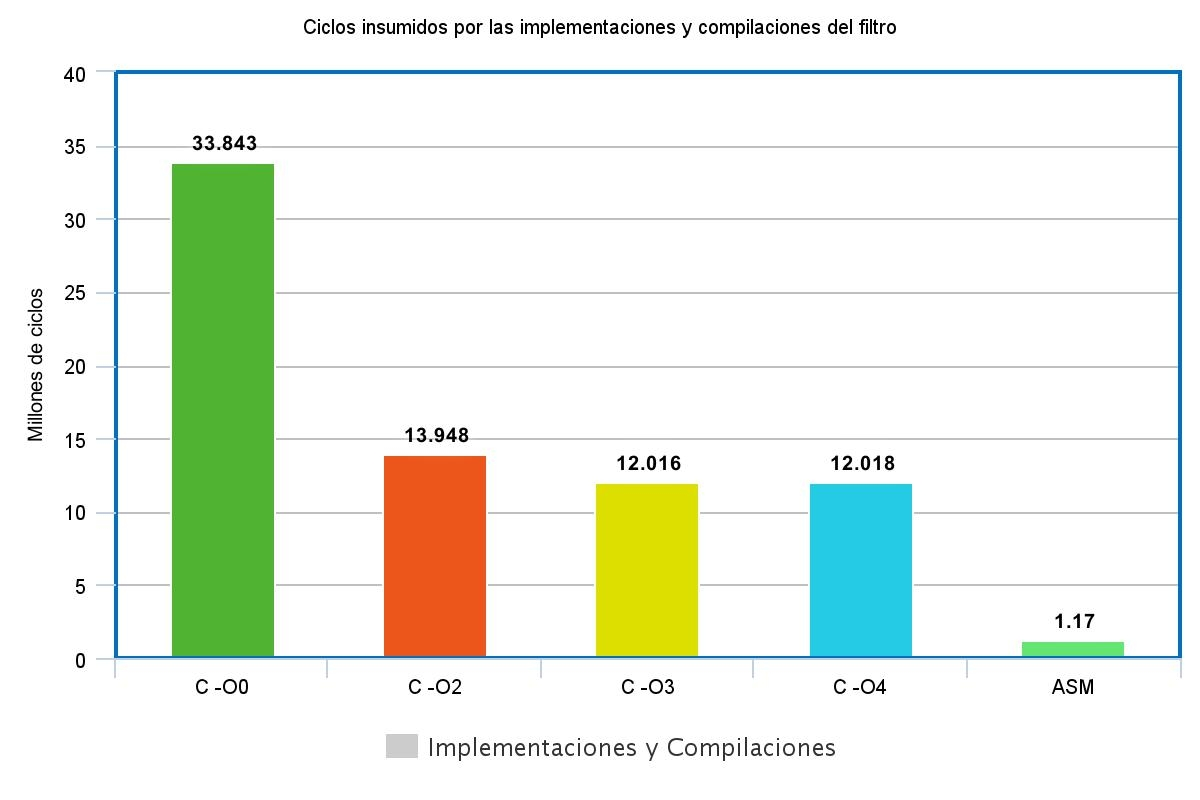
\includegraphics[width = 12 cm, height = 8 cm]{imagenes/CombinarASM-Cs.jpeg}
\end{figure}

\par{Como se puede apreciar, la implementación de ASM es casi 29 veces más rápida que la menos optimizada de C y también supera ampliamente a las optimizadas, siendo más de 10 veces más rápida. Esto confirma nuestras suposiciones de la mejoría resultante del modelo de procesamiento SIMD.}

\medskip

\par{Con respecto a lo planteado en cuanto a los accesos a memoria, también obtuvimos resultados esperados, visibles en la siguiente figura.}

\begin{figure}[h!]
\centering
	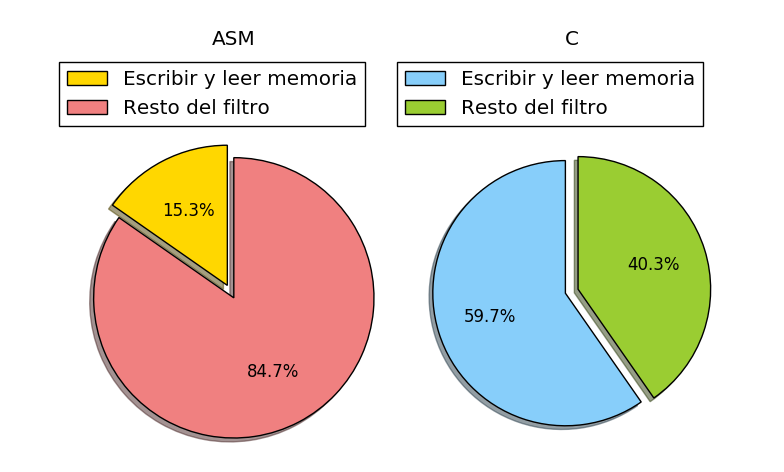
\includegraphics[width = 12 cm, height = 8 cm]{imagenes/CombinarMemoria.png}
\end{figure}

\par{A simple vista se observa que la implementación de ASM da como resultado que la mayor parte del tiempo de ejecución esté destinada al procesamiento de la imagen, al contrario de lo que ocurre con la implementación de C que resulta en un mayor consumo de ciclos por parte de los accesos a memoria.
\par{Más aún, el cociente entre el procesamiento de píxeles y los accesos a memoria para la implementación de ASM da 5,5, es decir que cada 13 ciclos, 11 surgen del procesamiento y 2 de los accesos. En cambio, este cociente es 0,68 para la implementación en C, de modo que la diferencia entre ambas implementaciones en cuanto al uso de la memoria y del procesador es muy significativa.}

\newpage
\section{Colorizar}

\subsection{Código C}
	El código C se trata de una conjuncion de ciclos, el exterior que recorre desde la segunda fila hasta la ante ultima,  y el interior que recorre desde la segunda columna hasta la ultima, dejando asi afuera a todos los bordes, tal como el enunciado pedia. \\ Luego en cada iteracion del ciclo interior, que es donde se hace las opearciones que modifican la imagen, lo que hacemos es crear un arreglo de unsinged chars, "res", que es  donde guardamos los maximos de cada canal en comparacion a todos  los pixeles lindantes del pixel en el cual estemos parado (una matriz de 3x3).
\begin{itemize}
\item {Res $[$0$]$ $\leftarrow$ MaximoLindantesAzul}
\item {Res $[$1$]$ $\leftarrow$ MaximoLindantesVerde}
\item {Res $[$2$]$ $\leftarrow$ MaximoLindantesRojo}
\end{itemize}
Luego con estos tres valores calculamos el alpha correspondiente de cada canal por el cual voy a multiplicar a cada uno. Y por ultimo reescribimos el pixel final, en la imagen src con cada canal multiplicado  por dicho alpha.

\subsection{Código ASM}
	El código en ASM se trata tambien de una conjuncion de ciclos. El recorre las filas desde la segunda hasta la ante ultima, y el interior recorre las columnas desde la segunda hasta la ante ultima, pero saltando de a dos pixeles, que es la cantidad que procesamos simultaneamente con instruccciones SSE. \\
	El ciclo interior consta de dos partes, la primera es calcular un registro en el que en las primeras dos DW guardamos los maximos valores de cada canal entre los pixeles lindantes, en sus posiciones respectivas. Se veria asi:\\
\ Vamos a hacer referencia como "fruta" cuando un byte tenga informacion que no nos interesa.
\par{\textbf{XMM1:}}
\xmmb{$Fruta$}{$Fruta$}{$Fruta$}{$Fruta$}{$Fruta$}{$Fruta$}{$Fruta$}{$Fruta$}{$A_M{p2}$}{$R_M{p2}$}{$G_M{p2}$}{$B_M{p2}$}{$A_M{p1}$}{$R_M{p1}$}{$G_M{p1}$}{$B_M{p1}$}
	
 Luego con esta informacion lo que hacemos es duplicar dicho registro y calcular el maximo de los maximos. Lo que hacemos para lograr esto es al registro duplicado	 lo shifteamos un lugar para la derecha, cosa de poder ir comparando entre ellos a los valores maximos de cada canal, y finalmente reproducimos el valor del maximo entre los maximos en todas las posiciones. El seguimiento de esta operacion seria la siguiente: 
\\Vamos a utilizar para esto los registros xmm1, y xmm2
\\
\par{\textbf{XMM2:}}
\xmmb{$Fruta$}{$Fruta$}{$Fruta$}{$Fruta$}{$Fruta$}{$Fruta$}{$Fruta$}{$Fruta$}{$A_M{p2}$}{$R_M{p2}$}{$G_M{p2}$}{$B_M{p2}$}{$A_M{p1}$}{$R_M{p1}$}{$G_M{p1}$}{$B_M{p1}$}
\par{\textbf{XMM1:}}
\xmmb{$Fruta$}{$Fruta$}{$Fruta$}{$Fruta$}{$Fruta$}{$Fruta$}{$Fruta$}{$Fruta$}{$A_M{p2}$}{$R_M{p2}$}{$G_M{p2}$}{$B_M{p2}$}{$A_M{p1}$}{$R_M{p1}$}{$G_M{p1}$}{$B_M{p1}$}
\par{shifteo un byte a la derecha xmm2 y hacemos pmaxub xmm1,xmm2  maximo entre ambos)}
\par{\textbf{XMM2:}}
\xmmb{$Fruta$}{$Fruta$}{$Fruta$}{$Fruta$}{$Fruta$}{$Fruta$}{$Fruta$}{$Fruta$}{$A_M{p2}$}{$R_M{p2}$}{$G_M{p2}$}{$B_M{p2}$}{$A_M{p1}$}{$R_M{p1}$}{$G_M{p1}$}{$B_M{p1}$}

\par{\textbf{XMM1:}}
\xmmb{$Fruta$}{$Fruta$}{$Fruta$}{$Fruta$}{$Fruta$}{$Fruta$}{$Fruta$}{$Fruta$}{$Fruta$}{$Fruta$}{$RG_M{p2}$}{$Fruta$}{$Fruta$}{$Fruta$}{$RG_M{p1}$}{$Fruta$}
\par {notar que varias casillas ahora tienen mas la asignacion de "fruta", y esto no es porque no sepamos que hay dentro de cada una, sino que no es informacion relevante a nuestras operaciones y que sera pisada si es necesario dentro de pronto}
\par{luego volvemos a shiftear y repetir la operacion pmaxub xmm1,xmm2  y queda: }

\par{\textbf{XMM2:}}
\xmmb{$Fruta$}{$Fruta$}{$Fruta$}{$Fruta$}{$Fruta$}{$Fruta$}{$Fruta$}{$Fruta$}{$A_M{p2}$}{$R_M{p2}$}{$G_M{p2}$}{$B_M{p2}$}{$A_M{p1}$}{$R_M{p1}$}{$G_M{p1}$}{$B_M{p1}$}

\par{\textbf{XMM1:}}
\xmmb{$Fruta$}{$Fruta$}{$Fruta$}{$Fruta$}{$Fruta$}{$Fruta$}{$Fruta$}{$Fruta$}{$Fruta$}{$Fruta$}{$Fruta$}{$RGB_{p2}$}{$Fruta$}{$Fruta$}{$Fruta$}{{\scriptsize $RGB_M{p1}$}}
\par{por ultimo con la instruccion pshuf, dejamos en xmm1 un registro con los maximos de los maximos representado de esta forma: }
\par{\textbf{XMM1:}}
\xmmb{$Fruta$}{$Fruta$}{$Fruta$}{$Fruta$}{$Fruta$}{$Fruta$}{$Fruta$}{$Fruta$}{$RGB_{p2}$}{$RGB_{p2}$}{$RGB_{p2}$}{$RGB_{p2}$}{{\scriptsize $RGB_M{p1}$}}{{\scriptsize $RGB_M{p1}$}}{{\scriptsize $RGB_M{p1}$}}{{\scriptsize $RGB_M{p1}$}}


	
	
   Y en la segunda parte del codigo lo que queda es que a este registro con la info del maximo de los maximos, lo transformamos en un registro con un 1 en el byte donde va el canal que contiene a este maximo entre los maximos (de cada pixel). Y ceros en el resto. \\ Teniendo esto ya,se puede apreciar en el codigo como nos armamos los alphas personalizados para cada pixel y terminamos multiplicandolos y reescribiendo ambos pixeles. \\
   Por ultimo avanzamos nuestros currents sobre columans en dos porque es la cantidad de pixeles que procesamos y  volvemos en caso de no haber terminado toda la fila a empezar el ciclo interior.
	
	
\subsection{Experimentación}
\subsubsection{Idea}	En la experimentacion de este filtro al igual que en el resto vamos a comparar el rendimiento respecto a los ciclos de clock, que tiene la funcion colorizar en C desde -o0 a -o3 contra asm. \\ Luego el segundo experimento va a consistir en probar la influencia del jump predictor en el codigo.\\ Primero agragando jumps de forma que no influya el flujo del programa solo para molestar al jump predictor.  Luego vamos a correrlo tal cual esta, y de apoco vamos a ir desenrollando el codigo. Como dijimos tiene un ciclo externo y uno interno, por lo que vamos a desenrrollar primero el interno 4 veces, despues 32 y ver que pasa.\\
Y finalmente el ultimo experimento que vamos a hacer es aprovechar el tamño que tiene el codigo y vamos a desenrrollarlo completamente, de manera que generemos un codigo tan grande que al correrlo no entre en la memoria cache para que el PC entonces empiece a generar Miss Hits en el momento de ir leyendo la proxima instruccion y ver que pasa entonces.
	   
\subsubsection{Hipótesis}
	Nuestra hipotesis es que el rendimiento va a ir mejorando a medida que vayamos cambiando los programas respectivamente a como los fui mencionando, osea el mas lento va a ser el codigo de asm, molestando al jmp predictor, y el mas rapido el desenrollando el codigo 32 veces. \\
	Y en el el ultimo test, por mas que desenrollemos todo el programa creemos justamente que va a ser el mas lento, por justamente el tamaño del codigo va a generar una gran cantidad de Miss Hits en lecturas de la siguiente instruccion, y que va a vencer la optimizacion generada por eliminar los controladores de flujo.	
	
\subsubsection{Resultados}
	Graficos lindos de lucia :D
	ciclos promedio colorizar c -o0 100 iteraciones : 101.898.160
	ciclos promedio colorizar c -o3 100 iteraciones : 21.567.776
	ciclos promedio colorizar original 1000 iteraciones: 5.980.263
	ciclos promedio colorizar JodiendoJumps1 1000 iteraciones: 5.977.453
	ciclos promedio colorizar Unrolling Ocho ciclos 100 iteraciones : 5.873.712
	
	
	
	ciclos promedio colorizar Unrolling lena 1024x768
	 todos los cilcos 100 iteraciones : 35.285.958
	
	ciclos promedio colorizar original lena 1024x768 100 iteraciones:	21.050.994
	
	
	
\subsubsection{Conclusión}
 Primera gran conclusión reveladora, c -o0 demuestra ser mucho mas lento que optimizando, el código mejoro 5 veces su cantidad de ciclos por llamada al compilar con -O3.
  Luego sin embargo la función hecha en  asm le sigue ganando por bastante a C, en una proporción de 3.5 veces mas rápido en cantidad de ciclos todavía.\\
  Ahora encuanto al experimento personalizado, hicimos una comparación con distintos códigos para medir la influencia del jump predictor en la ejecución del código. Primera prueba fue la de intentar molestar al Jump Predictor. Sin embargo por mas duro que itnentasemos, descubrimos que el algoritmo que lo dirige, es bastante mas sofisticado de lo que pensábamos, por lo que no pudimos influenciar en lo mas mínimo la eficiencia del código. \\
   Luego para contrastar el ultimo experimento mencionado, intentamos implementar lo contrario, desenrollar el código de manera que nunca influya un Miss Jump, en la ejecución del programa, sin embargo ya sacando la conclucion de lo mencionado recién, de que el sistema que lo regula es mas sofisticado del esperado, el desenrollar el código principal 4, y 32 veces, no estuvo mostrando ninguna diferencia con respecto al original. \\ 
   Por ultimo en el experimento final con desenrollar, en el cual se pretendia desenrollar completamente el codigo. Funciono muy bien, lo intentamos con una imagen mayor de lena, de 1024x768 para que el ciclo pueda ser desenrrollado mas cantidad de veces, y asi se ve que el codigo modificado tardo en promedio al rededor de unos 14.000.00 de ciclos mas que el original. Justamente por lo mencionado en la seccion de hipotesis que la cantidad de Miss Hits generados por el P.C tuvo mucha mayor influencia que el tema de los jumps.


\end{document}
